\section{Degenerate, tangent, and clipped traces}\label{sec:degenerate}

The stronger closed-section clause in \cref{thm:main} makes the boundary
cases explicit.

\begin{corollary}[Tangent and lower-dimensional trace preservation]
The construction preserves all of the following exactly.
\begin{enumerate}
\item If a prescribed line is tangent to a source neuron at a single closed
      point, the output has the same closed point contact and empty open
      trace.
\item If a supporting line meets a source closure in a nontrivial segment
      but misses the open field, the complete closed segment is retained and
      the strict trace remains empty.
\item If a source trace endpoint coincides with an ambient vertex, the
      clipped open trace may be half-open; its endpoint inclusion is
      unchanged.
\item Endpoint coincidences for several neurons remain simultaneous because
      every line section is retained as an actual subset, not merely through
      an order type.
\item Lower-dimensional atoms and closure-supported atoms remain codewords;
      any selected witness in such an atom is retained.
\end{enumerate}
\end{corollary}

\begin{proof}
The first two assertions follow from the exact closed- and open-section
identities.  The third follows because the complete bounded line section is
frozen before intersecting with the closed ambient polygon.  The fourth is
pointwise equality of several retained traces.  The last assertion follows
from exact code equality and \cref{cor:protected}.
\end{proof}

\begin{figure}[t]
\centering
\begin{subfigure}[t]{.46\textwidth}
\centering
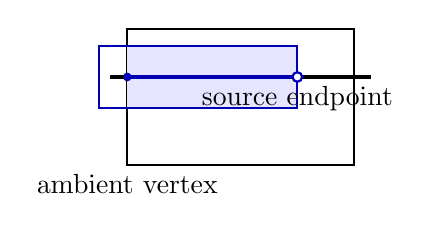
\begin{tikzpicture}[scale=.72]
  \draw[thick] (0,0) rectangle (4,2.4);
  \fill[blue!10] (0,1.0) rectangle (3,2.1);
  \draw[blue!70!black,thick] (-.5,1.0)--(3,1.0)--(3,2.1)--(-.5,2.1)--cycle;
  \draw[very thick] (-.3,1.55)--(4.3,1.55);
  \draw[blue!70!black,very thick] (0,1.55)--(3,1.55);
  \fill[blue!70!black] (0,1.55) circle (2.2pt);
  \draw[blue!70!black,fill=white,thick] (3,1.55) circle (2.4pt);
  \node[below] at (0,0) {ambient vertex};
  \node[below] at (3,1.55) {source endpoint};
\end{tikzpicture}

\caption{A globally open interval becomes half-open after clipping by an
ambient edge.}\label{fig:halfopen}
\end{subfigure}\hfill
\begin{subfigure}[t]{.46\textwidth}
\centering
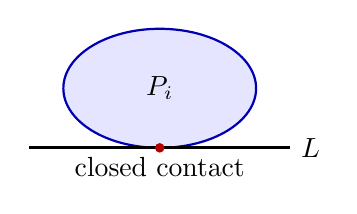
\begin{tikzpicture}[scale=.72]
  \fill[blue!10] (0,1.2) ellipse (1.7 and 1.05);
  \draw[blue!70!black,thick] (0,1.2) ellipse (1.7 and 1.05);
  \draw[very thick] (-2.3,.15)--(2.3,.15) node[right] {$L$};
  \fill[red!70!black] (0,.15) circle (2.4pt);
  \node[below] at (0,.15) {closed contact};
  \node at (0,1.2) {$P_i$};
\end{tikzpicture}

\caption{A tangent line has empty strict trace and a retained closed point
contact.}\label{fig:tangent}
\end{subfigure}
\caption{Boundary cases are controlled by recording complete line sections
before ambient clipping.}
\end{figure}

\begin{remark}[Empty and whole traces]
An empty trace requires no frame.  If the field contains the entire portion
of a prescribed line that meets $F$, the bounded auxiliary disk turns the
uncut trace into a compact interval that contains the clipped section in its
interior; the same argument applies.
\end{remark}

\begin{corollary}[Covered relative carriers]\label{cor:covered}
Suppose a specified subfamily of the source neurons covers
$\operatorname{int}F$.  The corresponding output polygons cover
$\operatorname{int}F$ as well.
\end{corollary}

\begin{proof}
The relative empty word with respect to that subfamily is absent from the
source code.  Exact relative code equality prevents it from appearing in the
output.  No approximation or Lebesgue-number argument is needed.
\end{proof}
